\section{System Architecture} \label{systemarch}
Our converting pipeline is subdivided into three main states: the \textbf{Import
Module}, the \textbf{Canonical Scene Representation} and the \textbf{Conversion
Module}, as illustrated in Figure \ref{fig:sysarch}. Given an arbitrary input
file format, our converter is able to import the scene and transform it into a
generic, canonical representation and then export it to different output
formats.

\begin{figure}[h]
\centering
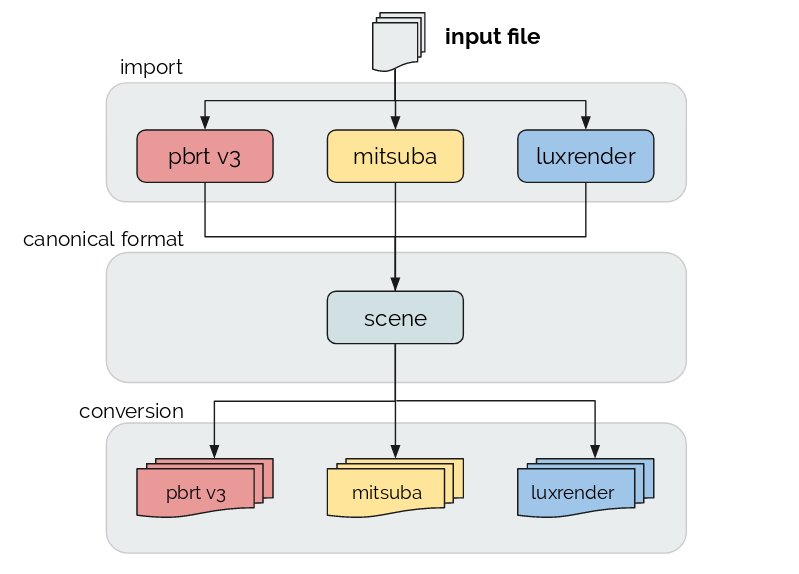
\includegraphics[width=3.5in]{figs/3_system_architecture/architecture.png}
\caption{Illustration of the system pipeline.}
\label{fig:sysarch}
\end{figure}

Our Proof of Concept (PoC) encompassed \textit{PBRT} \cite{pbrt}, \textit{Mitsuba}
\cite{mitsuba} and \textit{LuxRender} \cite{luxrender}, as these are three of
the most popularly used renderers in the community. This architecture, however,
is easily extensible: adding other renderers would be a simple task of writing
an import and a conversion module.

\subsection{Import Module}
Most physically-based renderers have a similar way of describing a scene.
Usually, they divide it into two sections: scene-wide rendering options and
world block. The former defines overall rendering settings (such as which
rendering or sampling technique should be used) while the latter describes the
geometry and which materials should be used for rendering.

Our import module specializes in reading and interpreting such scene files. The
input file is read, parsed and each directive is loaded into our canonical
representation. Since each renderer has its own proprietary file format, we have
developed three importing modules: one for each renderer.

\textit{PBRT} and \textit{LuxRender} file formats are composed of structured
text statements which define the directives. Given their structure, a Lex/Yacc
parser was considered the best choice for these formats. As we intended to keep
our system in pure Python, we chose to use PLY \cite{ply}, a Python
implementation of Lex and Yacc.

\textit{Mitsuba} is a heavily optimized, plugin-oriented renderer. The file
format is, essentialy, a XML description of which plugins should be instantiated
with the specified parameters. Since there are several
XML-parsing libraries for Python that can load the hierarchy into a tree data
structure, we didn't think it necessary to create a Lex/Yacc parser. We chose to
implement this module using ElementTree \cite{ET}, a Python XML parsing tool.

\subsection{Canonical Scene Representation}
After loading the scene file, the obtained information has to be
stored somewhere. While most renderers have the same base structure, they differ
in which parameters can be used to configure the techniques used during the
rendering process.

Renderer directives are usually given in the format of a command, followed by a
type and a list of additional parameters. So, for instance, to specify the path
integration technique with 8192 samples per pixel in \textit{PBRT} one would
write the following directive: \\ \\
\indent \textbf{Integrator ``path'' ``integer pixelsamples'' [8192]}\\

In order to establish a common ground for conversion, we decided it best to
define a canonical representation for these scenes. This representation can be
easily extended to incorporate any directives not contemplated in this work.

We divide the scene into \textbf{scene-wide rendering options} and \textbf{world
block}. The rendering options are divided into integration technique and sensor
options, while the world block is divided into lists of shapes, global emitters
and material definitions. This structure is illustrated in Figure
\ref{fig:canonicalrep}.

\begin{figure}[h]
\centering
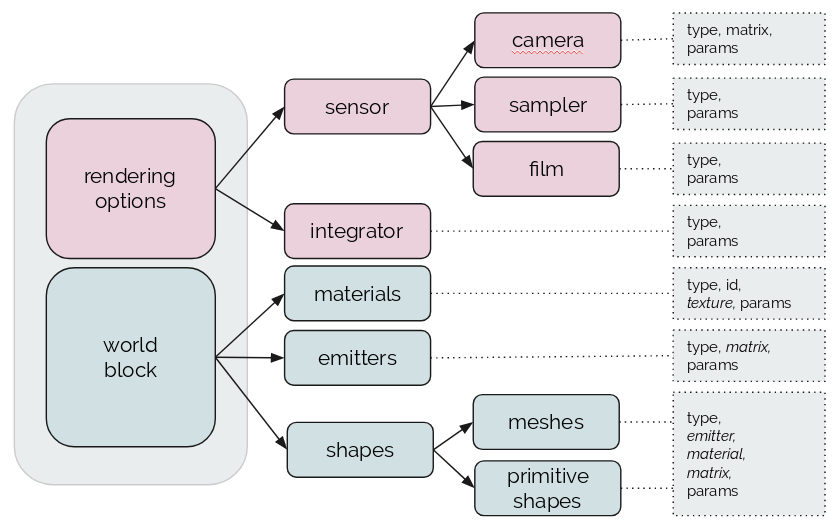
\includegraphics[width=3.5in]{figs/3_system_architecture/canonicalrep.png}
\caption{Illustration of the canonical scene representation.}
\label{fig:canonicalrep}
\end{figure}

\subsubsection{Scene-wide Rendering Options}
A set of directives specifying the integration and sampling techniques used for
rendering, camera and film properties. These directives are represented in a
structure with two fields: a type and a list of parameters.

\subsubsection{World Block}
A set of directives describing the shapes, materials and global emitters present
in the scene.

The \textbf{material} directive is represented in a structure with: a type, an
id, an optional texture and a list of parameters.

The \textbf{shape} directive is represented in a structure with: a type (cube,
sphere, ...), an optional area emitter, an optional material reference, an
optional transformation matrix and a list of parameters.

The \textbf{texture} directive is represented in a structure with: a type, an id and a list of parameters.

The \textbf{global emitter} directive is represented in a structure with: a
type, an optional transformation matrix and a list of parameters.

\subsection{Conversion Module}
After the scene file is loaded and properly set into our canonical
representation, it can be converted into any of the supported formats.

When converting scene representations, there are several delicate cases to
consider and study carefully. The matrix transformations, the native shape
directives, the environment mapping coordinates and, mostly, the materials are
some of the directives that vary greatly between renderers. 

% \subsubsection{Converting Matrices}
\textit{1. Converting Matrices} \\
There are several issues to consider when converting matrices between renderers.
A few things we had to keep in mind were: does this renderer use a left or right
coordinate system? Does this renderer represent matrices in the scene file using
the inverse-transpose? How is the object-world transformation represented for
shapes?

Mitsuba uses a right-hand coordinate system, while PBRT and LuxRender use a
left-hand one. This meant that, when converting between Mitsuba and the other
two, we had to mirror the x-axis of all camera matrix transformations. This was
also the case for environment mapping positioning and object-world
transformations.

\green{Furthermore, Mitsuba scene files have their camera position specified as a 
world-to-camera transformation matrix, while PBRT and LuxRender scene files have 
theirs as a camera-to-world transformation matrix. Therefore, converting the 
camera positioning between Mitsuba and the other two renderers means we have to 
compute the inverse transpose of this transformation matrix.}

% \red{Mitsuba also has its camera transformation matrix specified as a camera-to-world
%  transformation, while PBRT and LuxRender do not. Therefore, when converting the
% camera look-at matrix between these renderers, we had to compute the inverse
% transpose of the specified matrix. }

% \subsubsection{Converting Materials}
\textit{2. Converting Materials} \\
Materials are maybe the most delicate aspect of scene conversion. Materials have
spectral and roughness properties that absolutely must be gotten right when
converting scenes. However, most renderers have very different implementations
for common subsurface scattering models (called BSDFs), making it hard to
predict the relation between their parameters.

Mitsuba uses a more physics-oriented approach: a material can be diffuse,
conductor, dielectric, plastic, translucent, or a bumpmap.
There are other types of materials, but those were not contemplated in our PoC.
The material type in Mitsuba changes should the material contain any form of
surface roughness, becoming a ``rough'' version of itself (for instance, a rough
metal becomes a roughconductor).

PBRT and LuxRender materials have roughness parameters, making it unecessary to
change the material's name.

The major problem was faced when converting metals from and to LuxRender. PBRT 
and Mitsuba use the index of refraction ($\eta$) and the absorption 
coefficient (\textit{k}) in each channel in order to compute material's 
reflectance. LuxRender, however, uses a Fresnel texture, which can specify a 
single value of $\eta$ and \textit{k} for all channels, or specify an RGB 
color. Therefore, getting a converted metal color between LuxRender and the 
others is very difficult, and was not implemented for this PoC. \\

\textit{3. Converting Shapes} \\
Shape directives can be split into two categories: primitive shapes, which can
be used to specify simple geometry such as cubes, rectangles, spheres and disks;
and 3D meshes in external files.

Converting meshes between renderers is simple, as all of them have directives
for this exact purpose. However, PBRT does not support Object File Wavefront 3D
(.obj) files - these must be converted by the user with mesh converting tools.
Our system issues a warning, making the user aware of this problem.

Native shapes are more complex. Mitsuba has primitives for both cubes and
rectangles, while PBRT and LuxRender do not. The primitive defines canonical,
unitary points for these shapes, which can be modified with a transformation
matrix. These directives can be reproduced in PBRT and LuxRender using their
primitive for specifying inbuilt triangle meshes.

The reverse process, however, is more complicated. The triangle mesh directive
specifies the coordinates, normal and uv mapping for the points forming a
triangle. In order to recover a transformation matrix for the corresponding
Mitsuba primitive, \red{these points have to be multiplied by the original Mitsuba
canonical coordinates in the correct order.}

\textit{4. Converting Global Emitters} \\
Global emitters can used to emulate environment lighting, such as the sun, the
sky or even environment mapping. Converting these emitters can be tricky, mainly
because renderers don't implement the same algorithms and directives. For
instance, Mitsuba and LuxRender implement sun and sky algorithms; PBRT doesn't.
However, these directives can be converted from Mitsuba and LuxRender to PBRT. A
sun directive can be simulated in PBRT with a distant light. A sky directive can
be simulated using an environment mapping of a clear sky.

The inverse conversion can be a bit tricky. Converting a PBRT distant light into
a sun directive is a very straightforward conversion. Converting a PBRT
environment mapping into a sky directive is not: how could the converter know
whether the environment mapping is in fact an adaptation of a sky light? We
solved this issue by interacting with the user whenever an environment map
directive is found - we ask the user whether (s)he would like to use a sky
emitter or not.

Another sensitive point to consider is converting environment mapping 
indexation. In PBRT and LuxRender, environment maps' uv coordinates are indexed 
using spherical coordinates (\textit{theta} and \textit{phi}). Meanwhile, 
Mitsuba uses Cartesian coordinates (\textit{x}, \textit{y} and \textit{z}), as 
shown in \ref{fig:mitdocemitter}. 

\begin{figure}[h]
\centering
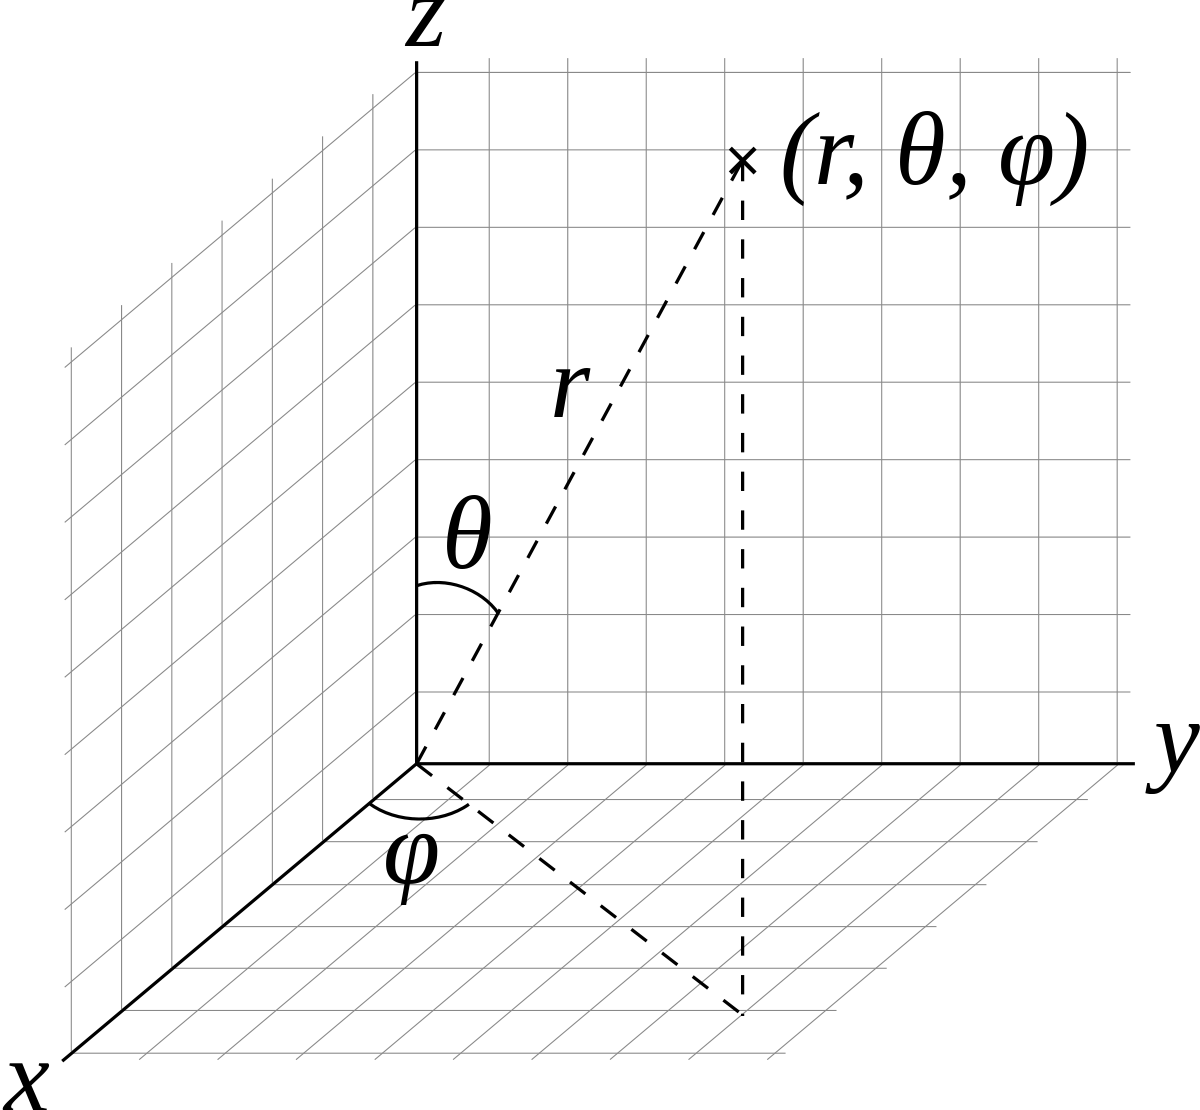
\includegraphics[width=1.4in]{figs/3_system_architecture/spherical_coordinates.png}
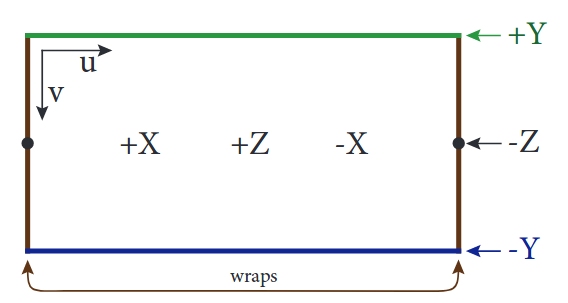
\includegraphics[width=2.2in]{figs/3_system_architecture/mitdocemitter.png}
\caption{Illustration of the coordinate conventions used by PBRT and LuxRender 
(top) and by Mitsuba (bottom) for indexing environment map uv coordinates.}
\label{fig:mitdocemitter}
\end{figure}

This conversion can be done by applying a transformation matrix on the 
environment map, rotating the x, y and z axes to match the output renderer. 